\documentclass{article}
\textheight 23.5cm \textwidth 15.8cm
%\leftskip -1cm
\topmargin -1.5cm \oddsidemargin 0.3cm \evensidemargin -0.3cm
%\documentclass[final]{siamltex}

\usepackage{verbatim}
\usepackage{fancyhdr}
\usepackage{amssymb,ctex}
\usepackage{mathrsfs}
\usepackage{latexsym,amsmath,amssymb,amsfonts,epsfig,graphicx,cite,psfrag}
\usepackage{eepic,color,colordvi,amscd}
\usepackage{enumerate}
\usepackage{enumitem}
\usepackage{booktabs}
\usepackage{graphicx}
\usepackage{float}
\usepackage{wrapfig}
\usepackage{multirow}
\usepackage{subfigure}
\usepackage{diagbox}
\usepackage{wasysym}

\title{USTC\_CG HW4 MinSurMeshPara}
\author{张继耀,PB20000204}

\begin{document}
	\maketitle
	
	\tableofcontents
	
	\section {问题介绍}
	\subsection{主要目的}
	
	\begin{itemize}
		\item 初步理解*.obj数据(*.obj,*.mtl)
		  \begin{itemize}[label=$\circ$, itemjoin=\hspace{0.5em}]
			\item 安装MeshLab查看三维数据文件
		\end{itemize}
	\end{itemize}
	
	\begin{itemize}
		\item 学习网格的数据结构及操作
		  \begin{itemize}[label=$\circ$, itemjoin=\hspace{0.5em}]
			\item 使用MeshFrame框架
		    \item 寻找非封闭网格曲面的边界
		\end{itemize}
	\end{itemize}
	
	\begin{itemize}
	\item 实现极小曲面与网格参数化
	\begin{itemize}[label=$\circ$, itemjoin=\hspace{0.5em}]
		\item 极小曲面:边界固定,求解方程组
		\item 参数化:边界映射到平面,求解方程组
	\end{itemize}
\end{itemize}
	
	\begin{itemize}
		\item 巩固使用Eigen库求解稀疏线性方程组
	\end{itemize}

    \subsection{实验内容}
    
    \begin{itemize}
    	\item  极小化曲面类:MinSurf.h 和 MinSurf.cpp,在其中完成极小曲面对应的算法。
    \end{itemize}

    \begin{itemize}
	\item  参数化类:Paramaterize.h 和 Paramaterize.cpp ,在其中完成网格参数化算法,并要求实现
	\begin{itemize}[label=$\circ$, itemjoin=\hspace{0.5em}]
		\item Uniform weight 
		\item Cotangent weight
		\item 显示纹理映射结果
	\end{itemize}
    \end{itemize}

\begin{itemize}
	\item  在UEngine中添加功能,主要有
	\begin{itemize}[label=$\circ$, itemjoin=\hspace{0.5em}]
		\item 求给定边界的极小曲面
		\item 非封闭网格曲面的参数化(圆形边界和正方形边界,两种权重的选取)
		\item 显示纹理映射
	\end{itemize}
\end{itemize}


	\section{算法设计}
	
	\subsection{极小曲面}
	
	考虑曲面的微分坐标,即
	$$ \delta_i = \nu_i -  \sum\limits_{\nu \in N(j)}\omega_j \nu_j  $$
	
	这里$N(i)$是和$\mu_i$相连的所有顶点的下标,$\omega_j$为权重,在求极小曲面的时候取了$\omega_j=  \frac{1}{d_j}$,这里$d_j$是顶点的度。
	
	为了方便起见,可直接规定$\sum \omega_i = 1 $。对于极小曲面,有$\delta_i = 0$成立。而边界上的点是固定不动的,于是我们得到线性方程组:
	
		$$ \left\{ 
	\begin{array}{lc}
		Lx=\delta=0   \\
		x_i=\nu_i  \enspace on  \enspace  Boundary   \\
	\end{array}
	\right.$$
	
	其中$L=I-D^{-1}A$,且有
	
		$$ A_{ij}=\left\{ 
	\begin{array}{lc}
		1 , i \in N(j) \\
	    0 , otherwise     \\
	\end{array}
	\right.$$
	
		$$ D_{ij}=\left\{ 
	\begin{array}{lc}
		d_i , i=j  \\
		0, otherwise  \\
	\end{array}
	\right.$$
	
	于是这个问题就变成了与HW3中类似的问题。还是利用Eigen库来求解方程组。
	
	\subsection{参数化}
    
    参数化与极小曲面相比,只多了一步就是将边界固定到平面凸多边形(例如正方形或圆形)上。只需将边界点按顺序均匀的分布在边界上即可。
    
    定义嵌入:
    	$$\left\{ 
    \begin{array}{lc}
    	Wx=b_x \\
    Wy=b_y   \\
    \end{array}
    \right.$$
    
    其中
    $$ w_{ij}=\left\{ 
    \begin{array}{lc}
    	< 0 , (i,j)\in E   \\
    	-\sum_{j\ne i}\omega_{ij} ,(i,i) \\
    	0, otherwise 
    \end{array}
    \right.$$
    
    考虑如下两种权重:
    	\begin{itemize}
    	\item Uniform weight 
    		\begin{itemize}[label=$\circ$, itemjoin=\hspace{0.5em}]
    		\item $\omega_j$=1
 
    	\end{itemize}
    	\item Cotangent weight
    		\begin{itemize}[label=$\circ$, itemjoin=\hspace{0.5em}]
    		\item $\omega_j$=$(cot\alpha+cot\beta)$
    	\end{itemize}
    \end{itemize}

    剩下的步骤就与极小曲面的一样了。
    
  
	\section{结果展示}
	
	 \subsection{程序界面}
	 
	 \begin{figure}[H]
	 	\begin{center}
	 		
	 		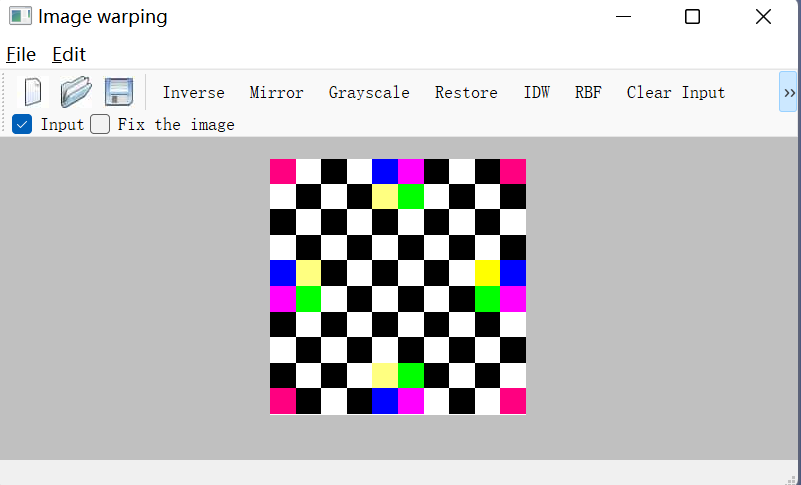
\includegraphics[width=11cm,height=6cm]{jiemian}
	 		
	 		\caption{程序界面} \label{jiemian.label}
	 	\end{center}
	 \end{figure}
 
  程序界面如上所示
   \begin{itemize}
 	\item  添加了两个按钮ParamaterizeShape和ParamaterizeWeight,用于选择参数化时边界的形状和选择的权重
   \end{itemize}

   \begin{itemize}
	\item  Paramaterize时完成参数化,ParamaterizeMesh时显示输出的结果
\end{itemize}
	 

	 
	      \subsection{实验结果}
	      
	  
    
     \subsubsection{测试样例}
    
    \begin{table}[htbp]
    	\centering
    	\setlength{\fboxsep}{0pt} % 重置图像的内边距
    	\begin{tabular}{|c|c|c|c|c|}
    		\hline
    		\diagbox[width=3cm]{\textbf{测试例子}}{\textbf{使用方法}} & \textbf{原图} & \textbf{极小曲面} & \textbf{纹理(Uniform参数化)} & \textbf{纹理(CoTan参数化)} \\
    		\hline
    		\multirow{2}{*}{\textbf{Ball}} & \raisebox{-0.5\height}{\includegraphics[width=2.5cm,height=2.5cm]{ballyuan.png}} & \raisebox{-0.5\height}{\includegraphics[width=2.5cm,height=2.5cm]{ballmin.png}} & \raisebox{-0.5\height}{\includegraphics[width=3cm,height=2.5cm]{ball uni wenli.png}} & \raisebox{-0.5\height}{\includegraphics[width=2.5cm,height=2.5cm]{ball cot wenli.png}} \\
    		
    		& & & & \\
    		\hline
    		\multirow{2}{*}{\textbf{Bunny Head }} & 	\raisebox{-0.5\height}{\includegraphics[width=2.5cm,height=2.5cm]{rabyuan.png}} & \raisebox{-0.5\height}{\includegraphics[width=2.5cm,height=2.5cm]{rabmin.png}} & \raisebox{-0.5\height}{\includegraphics[width=3cm,height=2.5cm]{rab uniwenli.png}} & \raisebox{-0.5\height}{\includegraphics[width=3cm,height=2.5cm]{rab cotwenli.png}} \\
    		
    		
    		
    		& & & & \\
    		\hline
    		
    		\multirow{2}{*}{\textbf{  Cat Head}} & \raisebox{-0.5\height}{\includegraphics[width=2.5cm,height=2.5cm]{catyuan.png}} & \raisebox{-0.5\height}{\includegraphics[width=2.5cm,height=2.5cm]{catmin.png}} & \raisebox{-0.5\height}{\includegraphics[width=3cm,height=2.5cm]{cat uni wenli.png}} & \raisebox{-0.5\height}{\includegraphics[width=3cm,height=2.5cm]{cat cot wenli.png}} \\
    		
    		& & & & \\
    		\hline
    		
    		\multirow{2}{*}{\textbf{ David }} & \raisebox{-0.5\height}{\includegraphics[width=2.5cm,height=2.5cm]{daviyuan.png}} & \raisebox{-0.5\height}{\includegraphics[width=2.5cm,height=2.5cm]{davimin.png}} & \raisebox{-0.5\height}{\includegraphics[width=3cm,height=2.5cm]{daviuni.png}} & \raisebox{-0.5\height}{\includegraphics[width=3cm,height=2.5cm]{davicot.png}} \\
    		
    		
    		& & & & \\
    		\hline
    		
    		\multirow{2}{*}{\textbf{ Face }} & \raisebox{-0.5\height}{\includegraphics[width=2.5cm,height=2.5cm]{catyuan.png}} & \raisebox{-0.5\height}{\includegraphics[width=2.5cm,height=2.5cm]{catmin.png}} & \raisebox{-0.5\height}{\includegraphics[width=3cm,height=2.5cm]{cat uni wenli.png}} & \raisebox{-0.5\height}{\includegraphics[width=3cm,height=2.5cm]{cat cot wenli.png}} \\
    		
    		
    		& & & & \\
    		\hline
    	\end{tabular}
    	\caption{主要结果}
    \end{table}
	         
	         \subsubsection{两种参数化的对比}
	         
	         以下是测试两种参数化在映射到圆形边界或正方形边界的例子,第一个表格是对Ball做的测试
	         
	         	\begin{table}[h]
	         	\centering
	         	\begin{tabular}{|c|c|c|}
	         		\hline
	         		\diagbox[width=3cm]{\textbf{使用方法}}{\textbf{边界形状}} & \textbf{正方形} & \textbf{圆形} \\
	         		\hline
	         		\multirow{2}{*}{\textbf{Uni}} & \raisebox{-0.5\height}{\includegraphics[width=3cm,height=3cm]{ball uni rect.png}} & \raisebox{-0.5\height}{\includegraphics[width=3cm,height=3cm]{ball uni circle.png}} \\
	         	
	         		& & \\
	         		\hline
	         		\multirow{2}{*}{\textbf{Cot}} & \raisebox{-0.5\height}{\includegraphics[width=3cm,height=3cm]{ball cot rect.png}} & \raisebox{-0.5\height}{\includegraphics[width=3cm,height=3cm]{ball cot circle.png}} \\
	         	
	         		& & \\
	         		\hline
	         	\end{tabular}
	         	\caption{对Ball做的测试结果}
	         \end{table}
         
         人脸的例子可能会更明显一些。可以看出Cot方式基本能看出清晰的轮廓,Uni方式就要差一些。
         
         	\begin{figure}
         	\begin{minipage}[H]{0.5\linewidth}
         		\centering
         		\includegraphics[scale=0.35]{face uni rect.png}
         		\caption{Uni方式}
         	\end{minipage}%
         	\begin{minipage}[H]{0.5\linewidth}
         		\centering
         		\includegraphics[scale=0.35]{face cot rect.png}
         		\caption{Cot方式}
         	\end{minipage}
         \end{figure}
         
	
	\section{总结与讨论}
	
	   \begin{itemize}
		\item  通过选取不同的权重和边界条件,参数化的结果也是不同的。可以看到,Cot方式一般会比Uni方式要好一些。通常来说,Cot方式产生的图像纹理更平整、光滑。
	\end{itemize}

   \begin{itemize}
	\item  在人脸映射时,正方形边界有时会出现缺角的情况,这可能是由于映射到边界时是均匀映射过去的。如果对正方形的四个顶点做特殊处理可能会解决掉,但时间关系来不及做了。
\end{itemize}

   \begin{itemize}
	\item  在写参数化时,可以调用极小曲面已有的函数来得到结果,代码会更简洁一些。
\end{itemize}
	

\end{document}